\zotelo{../thesis.bib}

\chapter{Particle-in-Cell Simulation}
\label{chap:pic}

\section{Introduction}
\label{sec:introduction}

The Particle-in-Cell(PIC) technique is a powerful tool to study the kinetic
properties of plasma from first principles. The strength of a PIC code is that
it can resolve the plasma skin depth, and reproduce the interaction between
particles and fields, making them invaluable in the study of particle
acceleration processes in plasmas. Also it is relatively straight-forward to
implement and easily parallelizable. It has been very successfully applied to
collisionless shocks and reconnection processes in astrophysics
%% TODO: references
. However, because a PIC code has to resolve the
plasma skin depth which is usually many orders of magnitude smaller than the
scale of a realistic astrophysical problem, this kind of simulation is extremely
expensive and very often only applied to local problems to study the
microphysics in a relatively large system.

This chapter introduces the PIC technique in detail, and then introduces
Aperture, a versatile PIC code designed and developed from scratch as part of my
PhD thesis. The name is a recursive acronym which stands for ``Aperture is a code
for Particles, Electrodynamics and Radiative Transfer at Ultra-Relativistic
Energies''. The original and main purpose of the code was to simulate the global
structure of the Pulsar magnetosphere from first principles. However, we
designed the code to be general enough to be applied to many different problems
in Astrophysics, especially in problems where particles are accelerated in
strong magnetic fields and capable of producing pair cascade.

% TODO: Update this paragraph
In Section \ref{sec:particle-cell-method} of the paper we will present
the numerical algorithms and techniques employed in the Aperture code,
from coordinate systems to boundary conditions. In Section
\ref{sec:test-problems} we will present some simple test cases to show
the validity of the code. Finally in Section
\ref{sec:example-applications} we will present some of the problems
that we can address using this new PIC code.

\section{The Particle-in-Cell Method}
\label{sec:particle-cell-method}
% This section is the meat of this paper. There will probably be many
% subsections.
The PIC method is essentially a way to solve the coupled Maxwell-Vlasov
equations by approximating the plasma distribution function using the
sum of a large number of discrete macro-particle distributions. The
system of equations under question is simply the Maxwell equations
combined with the Vlasov equation:
\begin{align}
  \frac{\partial f^{s}}{\partial t} + \mathbf{u}\cdot\frac{\partial f^s}{\partial \mathbf{x}} &+ \frac{q^s}{m^s}\left(\mathbf{E} + \frac{\mathbf{u}}{c}\times \mathbf{B}\right)\cdot\frac{\partial f^s}{\partial (\gamma \mathbf{u})} = 0 \label{eq:vlasov}\\
  \nabla\cdot \mathbf{E} &= 4\pi\rho \\
  \nabla\cdot \mathbf{B} &= 0 \\
  \nabla\times \mathbf{E} &= -\frac{1}{c}\partial_t \mathbf{B} \\
  \nabla\times \mathbf{B} &= \frac{1}{c}\partial_t \mathbf{E} + \frac{4\pi}{c} \mathbf{j}
\end{align}
where $s$ denotes the particle species (electrons, positrons, ions,
\dots). We assume a collisionless plasma by setting the right hand
side of equation \eqref{eq:vlasov} to zero, which is applicable for a lot of
astrophysical applications.

The charge and current densities appearing in the Maxwell equations as source
terms are found by taking the moments of the distribution function $f^s$ over
the momentum space
\begin{align}
  \rho &= \int d \mathbf{u} \sum_s q^s f^s(\mathbf{x}, \mathbf{u}) \label{eqn:pic-rho} \\
  \mathbf{j} &= \int d \mathbf{u} \sum_s q^s \mathbf{u} f^s(\mathbf{x}, \mathbf{u}) \label{eqn:pic-j}
\end{align}
Macro particles are introduced to sample the distribution function $f^s$ in both
position and momentum space. We approximate the distribution function of each
species by sampling it with a finite but large number of macro particles each
with a smeared out distribution in space but identical momentum
$\mathbf{p}_{p}$:
\begin{equation}
  \label{eq:single-particle}
  f^s(\mathbf{x}, \mathbf{u}) = \sum_{p}f^s_{p}(\mathbf{x}, \mathbf{u}) = \sum_{p}\delta(\gamma m_{p}\mathbf{u} - \mathbf{p}_{p}) S(\mathbf{x} - \mathbf{x}_{p})
\end{equation}
% A macro particle can be
% viewed as a collection of particles smeared out in space, with
% identical physical momentum $\mathbf{p}_{p}$. Therefore, each
% particle represents a distribution function of the type
where $S$ is a function that describes the shape of the macro particle, with the
property that $S$ has finite support, and that the integral of $S$ over all
space is normalized to 1. Since the Vlasov equation is linear, if each
individual macro particle satisfies the Vlasov equation, then the linear
superposition of a large number of them still satisfy the Vlasov equation, and
should provide a good approximation for the dynamics of the plasma.

The dynamic equations for the macro particles can be derived by taking
the moments of the Vlasov equation with the single particle
distribution function \eqref{eq:single-particle}. Plugging the single
particle distribution function into the Vlasov equation and taking the
zeroth moment by integrating over $\mathbf{u}$, we get
\begin{equation}
  \begin{split}
    \int d\mathbf{u}\,\left\{ \left[ \partial_t \delta(\gamma m_{p}\mathbf{u} - \mathbf{p}_p) \right]S(\mathbf{x} - \mathbf{x}_p) + \delta(\gamma m_{p}\mathbf{u} - \mathbf{p}_p)\partial_tS(\mathbf{x} - \mathbf{x}_p) \right. \\
    + \delta(\gamma m_{p}\mathbf{u} - \mathbf{p}_p) \mathbf{u}\cdot\nabla S(\mathbf{x} - \mathbf{x}_p) \\
    \left. + S(\mathbf{x} - \mathbf{x}_p)\frac{q_p}{m_p}\left(\mathbf{E} +
        \frac{\mathbf{u}}{c}\times \mathbf{B}\right)\cdot \nabla_{\gamma
        \mathbf{u}}\delta(\gamma m_{p}\mathbf{u} - \mathbf{p}_p) \right\} = 0
  \end{split}
\end{equation}
The first term is an integral of the derivative of a delta function,
which should give zero since $S$ is independent of the integrand. The
second and third term can be integrated trivially to get
\begin{equation}
  \label{eq:eom-position}
\frac{d\mathbf{x}_p}{dt} = \mathbf{u}_p = \frac{\mathbf{p}_p}{\gamma_p m_{p}}
\end{equation}
The reason is that $\mathbf{x}_p$ depends only on $t$, therefore
the partial derivative becomes a total derivative,
$\partial_tS(\mathbf{x} - \mathbf{x}_p) = -\nabla
S(\mathbf{x} - \mathbf{x}_p) \cdot d\mathbf{x}_p/dt$. The
last term which involves the electromagnetic force requires a bit more
attention. The $\mathbf{E}$ field term again integrates to zero
since it is an integral of the derivative of a delta function. The
Lorentz force term needs an integration by parts, but then it would
become zero because $\nabla_{\gamma
  \mathbf{u}}\cdot(\mathbf{u}\times \mathbf{B})$ is zero.

% The dynamic equations for the macro particles can be derived by taking
% the moments of the Vlasov equation with the single particle
% distribution function \eqref{eq:single-particle}. It turns out that
% these dynamic equations are identical to the equations of motion of a
% single particle in electromagnetic field:
% \begin{align}
%   \label{eq:particle-equations}
%   \frac{d\mathbf{x}_p}{dt} = \mathbf{u}_p = \frac{\mathbf{p}_p}{\gamma_p} \\
%   \frac{d\mathbf{p}_p}{dt} = \frac{q_p}{m_p}(\mathbf{E} + \mathbf{u}_p\times \mathbf{B})
% \end{align}
% Therefore it is justified to treat macro particles as their name
% suggests: simply as physical particles. The code simply trace their
% motion in the electromagnetic field as described by the above dynamic
% equations.

Taking the first moment of the Vlasov equation yields
\begin{equation}
\begin{split}
    \int d\mathbf{u}\,\left\{ \mathbf{u}\left[ \partial_t \delta(\gamma m_{p}\mathbf{u} - \mathbf{p}_p) \right]S(\mathbf{x} - \mathbf{x}_p) + \mathbf{u}\delta(\gamma m_{p}\mathbf{u} - \mathbf{p}_p)\partial_tS(\mathbf{x} - \mathbf{x}_p) \right. \\
    + \mathbf{u}\delta(\gamma m_{p}\mathbf{u} - \mathbf{p}_p) \mathbf{u}\cdot\nabla S(\mathbf{x} - \mathbf{x}_p) \\
    \left. + \mathbf{u}S(\mathbf{x} - \mathbf{x}_p)\frac{q_p}{m_p}\left(\mathbf{E} + \frac{\mathbf{u}}{c}\times \mathbf{B}\right)\cdot \nabla_{\gamma \mathbf{u}}\delta(\gamma m_{p}\mathbf{u} - \mathbf{p}_p) \right\} = 0
\end{split}
\end{equation}
The second and third terms give the same equation of motion as above, and they
are proportional to the gradient of $S$, independent of the other two terms,
therefore we ignore them. The rest two terms can be reduced to the simple
single-particle equation of motion:
\begin{equation}
  \label{eq:eom-momentum}
\frac{d\mathbf{p}_p}{dt} = q_p\left(\mathbf{E} + \frac{\mathbf{u}_{p}}{c}\times \mathbf{B} \right)
\end{equation}

These are simply equations of motion for ordinary particles in an
electromagnetic field. Therefore it is justified to treat macro particles as
their name suggests: simply as physical particles. A PIC code simply trace their
motion in the electromagnetic field as described by the above dynamic equations.


\subsection{Discretization and Spatial Grid}
\label{sec:discretization}

So far the only approximation we have introduced is using an ensemble of macro
particles to approximate the real distribution function of a plasma system. To
solve the Maxwell equations and particle dynamic equations numerically, one
needs to discretize the continuous field quantities onto a finite grid
consisting of cells, hence the name Particle-in-Cell. The discretization is done
on space and time using the Finite Difference Time Domain (FDTD)
method. %TODO: Reference?
Fields $\mathbf{E}$ and $\mathbf{B}$ are sampled on a finite grid, as well as
the current and charge densities $\mathbf{J}$ and $\rho$. One evolves the
equations using a given time evolution scheme step by step starting from the
initial condition. At each step, one updates the positions and momenta of all
particles according to the fields on the grid, computes the current density due
to particle motion, and uses this current density to evolve the fields
themselves.

A PIC code can operate in either 2D or 3D\footnote{In 1D, a discretization is
  not necessary, since there is no magnetic field, and electric field at any
  given particle location can be found exactly by integrating Gauss's law.}.
In the former case, although a grid of lower dimension is used, all 3 vector
components of $\mathbf{E}$ and $\mathbf{B}$ fields need to be
evolved\footnote{A code like this is sometimes called ``2.5D'' due to full 3D vector quantities
  defined on a 2D grid.}. This is applicable when the problem has inherent
symmetry, such as axisymmetry or translational invariance in one direction. It
is typical to use the classical staggered \citet{yee_numerical_1966} grid for
electric and magnetic fields (figures \ref{fig:Yee} and
\ref{fig:Yee-cartesian}).

\begin{figure}[h]
  \centering
  \begin{tikzpicture}[label distance=-2.5mm]
    \begin{scope}[scale=1.3]
      \draw[->] (-0.5, 0) -- node[left] {$r$} (-0.5, 2);
      \draw[->] (0, -0.5) -- node[below] {$\theta$} (2, -0.5);
      \draw[dashed] (0,0) rectangle (3,3);
      \node [label=below:$\rho\text{, }j_{\phi}\text{, }E_{\phi}$] (center) at (1.5,1.5) {$\times$};
      \node [label=right:$j_{\theta}\text{, }E_\theta\text{, }B_{r}$] (right) at (3,1.5) {$\times$};
      \node [label=above:$j_r\text{, }E_r\text{, }B_{\theta}$] (top) at (1.5,3) {$\times$};
      \node [label=right:$B_\phi$] (top right) at (3,3) {$\times$};
    \end{scope}
  \end{tikzpicture}
  \caption{Staggered Yee cell for a 2D spherical grid.}
  \label{fig:Yee}
\end{figure}

\begin{figure}[h]
  \centering
  \begin{tikzpicture}[label distance=-2.5mm]
    \begin{scope}[scale=1]
      \pgfmathsetmacro{\l}{4}
      \pgfmathsetmacro{\h}{2}
      \pgfmathsetmacro{\d}{0.8}
      \draw[dashed] (0, 0, 0) -- ++(\l, 0, 0);
      \draw[dashed] (0, 0, 0) -- ++(0, \l, 0);
      \draw[dashed] (0, 0, 0) -- ++(0, 0, \l);
      \draw[thin] (0, 0, \l) -- ++(\l, 0, 0) -- ++(0, 0, -\l)
      -- ++(0, \l, 0) -- ++(-\l, 0, 0) -- ++(0, 0, \l) -- cycle;
      \draw[thin] (\l, \l, \l) -- ++(-\l, 0, 0);
      \draw[thin] (\l, \l, \l) -- ++(0, -\l, 0);
      \draw[thin] (\l, \l, \l) -- ++(0, 0, -\l);
      \draw[very thick, ->, red] (\h, \l, \h) node[right] {$B_{z}$} -- ++(0, \d, 0);
      \draw[very thick, ->, red] (\h, \h, \l) node[below] {$B_{x}$} -- ++(0, 0, -\d);
      \draw[very thick, ->, red] (\l, \h, \h) node[below] {$B_{y}$} -- ++(\d, 0, 0);
      \draw[very thick, ->, blue] (0, \h, \l) node[left] {$j_{z},\ E_{z}$} -- ++(0, \d, 0);
      \draw[very thick, ->, blue] (\h, 0, \l) node[below] {$j_{y},\ E_{y}$} -- ++(\d, 0, 0);
      \draw[very thick, ->, blue] (\l, 0, \h) node[below right] {$j_{x},\ E_{x}$} -- ++(0, 0, -\d);
      \node[label=below left:$\rho$] at (0, 0, \l) {};

      \draw[->] (-3, -3, 0) -- (1, -3, 0) node[below] {$y$};
      \draw[->] (-3, -3, 0) -- (-3, 1.2, 0) node[left] {$z$};
      \draw[->] (-3, -3, 0) -- (-3, -3, 3) node[above left] {$x$};
      % \draw (0,0,0) rectangle (3,0,3);
      % \draw (0,0,0) rectangle (0,3,3);
      % \node [label=below:$\rho\text{, }j_{\phi}\text{, }E_{\phi}$] (center) at (1.5,1.5) {$\times$};
      % \node [label=right:$j_{\theta}\text{, }E_\theta\text{, }B_{r}$] (right) at (3,1.5) {$\times$};
      % \node [label=above:$j_r\text{, }E_r\text{, }B_{\theta}$] (top) at (1.5,3) {$\times$};
      % \node [label=right:$B_\phi$] (top right) at (3,3) {$\times$};
    \end{scope}
  \end{tikzpicture}
  \caption{Staggered Yee cell for a 3D Cartesian grid.}
  \label{fig:Yee-cartesian}
\end{figure}

The reason for staggering the fields this way is that all derivatives that arise
in Maxwell equations will automatically have at least second order accuracy. For
example take the evolution of the $B_z$ term:
\begin{equation}
  % \label{eq:2}
  \begin{split}
    \frac{\Delta B_z(x, y)}{\Delta t} = -(\nabla\times \mathbf{E})_{z} = &-\left[ \frac{E_x(y + \Delta y/2) - E_x(y - \Delta y/2)}{\Delta y} \right. \\
      &- \left.\frac{E_y(x + \Delta x/2) - E_y(x - \Delta x/2)}{\Delta x} \right]
  \end{split}
\end{equation}
The electric field values needed show up exactly at where they are defined on
the Yee lattice, and due to the symmetric structure of the finite difference,
the $\Delta x^{2}$ term in the Taylor expansion naturally cancels:
\begin{equation}
  \label{eq:finite-diff-2nd-order}
\partial_xE_y = \frac{E_y(x + \Delta x/2) - E_y(x - \Delta x/2)}{\Delta x} + \mathcal{O}(\Delta x^3)
\end{equation}
This naturally applies to all derivative terms in the Maxwell equation.

Another strength of the Yee grid is that the differential relations
$\nabla\cdot(\nabla\times \mathbf{F}) = 0$ and $\nabla \times \nabla f = 0$ are
satisfied by construction, so as long as Maxwell equation is used for the
evolution of fields, $\nabla\cdot \mathbf{B} = 0$ should be preserved to
numerical precision without extra work.

This construction of symmetric finite difference scheme can be extended to
higher orders as well. Equation \eqref{eq:finite-diff-2nd-order} is accurate to
second order in $\Delta x$. To achieve 4th order accuracy, we need to use more
terms to cancel out the $\Delta x^{3}$ term in the Taylor expansion:
\begin{equation}
  \label{eq:finite-diff-4th-order}
  \partial_{x}E_y = \frac{2}{3}\frac{E_y(x + \Delta x/2) - E_y(x - \Delta x / 2)}{\Delta x} - \frac{1}{12}\frac{E_y(x + 3\Delta x / 2) - E_y(x - 3\Delta x / 2)}{\Delta x}
\end{equation}
Further


Macro-particles stream freely in the mesh grid, and their positions and momenta
are not discretized. To convert between local ``paticle'' quantities and grid
variables, an interpolation scheme is required. Fortunately we already have a
function $S(\mathbf{x} - \mathbf{x}_p)$ which describes the shape of the macro
particle smeared in space. Integrating equation \eqref{eqn:pic-rho} using a
macro particle distribution function over the volume of a cell gives:
\begin{equation}
  \label{eqn:rho-cell}
  Q_{c} = \rho_{c}\Delta V = \sum_pq_pW(\mathbf{x}_p-\mathbf{x}_{c})
\end{equation}
where $q_p$ is the charge of an individual macro particle, $\mathbf{x}_{c}$ is
the position of the center of the cell, and $W$ is defined as
the integral of $S$:
\begin{equation}
  \label{eqn:weight-function}
  W(\mathbf{x}_p - \mathbf{x}_c) = \int_{\mathbf{x}_c - \mathbf{\Delta}/2}^{\mathbf{x}_c + \mathbf{\Delta}/2} S(\mathbf{x}_p - \mathbf{x})d\mathbf{x}
\end{equation}
and $\Delta$ is the size of the cell. The assumption that $S$ has finite support
implies that $W$ will be nonzero for only a few cells with $\mathbf{x}_{c}$
close to $\mathbf{x}_{p}$, and since the integration of $S$ over the whole
volume is constrained to be 1, the sum of all nonzero $W$ near a certain
particle is guaranteed to be 1. This is another way of saying total charge is
conserved. Since in the PIC code, we will only be using the discrete
interpolation functions $W$, not $S$, so we will call $W(\mathbf{x}_p -
\mathbf{x}_c)$ the ``shape functions''. Typical shape functions used in PIC
codes are so-called ``B-spline'' functions, which are piecewise polynomial
functions with minimal support. Following are the shape functions often used in
PIC codes, in ascending polynomial order:

\textbf{CIC}: Cloud in Cell
\begin{equation}
    W^1(x) = \begin{cases}
        1 - |\delta| & \quad \text{if } |\delta| < 1, \\
        0            & \quad \text{otherwise}
    \end{cases}
\end{equation}

\textbf{TSC}: Triangular Shaped Cloud
\begin{equation}
    W^2(x) =
    \begin{cases}
        \frac{3}{4} - \delta^2 & \quad \text{if } |\delta| < 1/2, \\
        \frac{1}{2} \left( \frac{3}{2} - |\delta| \right)^2 & \quad \text{if } 1/2 \leq |\delta| < 3/2, \\
        0                      & \quad \text{otherwise}
    \end{cases}
\end{equation}

\textbf{PCS}: Piecewise Cubic Spline
\begin{equation}
    W^3(x) =
    \begin{cases}
        \frac{1}{6} \left( 4 - 6\delta^2 + 3|\delta|^3 \right) & \quad \text{if } |\delta| < 1, \\
        \frac{1}{6} \left( 2 - |\delta| \right)^3 & \quad \text{if } 1 \leq |\delta| < 2, \\
        0                      & \quad \text{otherwise}
    \end{cases}
\end{equation}

% TODO: insert a plot of these functions
In 2D or 3D problems, the weight of the particle is given by multiplication of
these shape functions, e.g.\ in 3D Cartesian coordinates $W(\mathbf{x}_{p} -
\mathbf{x}_{c}) = W(x_{p} - x_{c})W(y_{p} - y_{c})W(z_{p} - z_{c})$. In general,
higher order shape functions will have better noise properties for the result,
but are computationally more intensive, not only because they involve more
multiplications (higher order polynomial), but each particle can influence more
grid points and one need to sum over more terms of nonzero $W$.

Equation \eqref{eqn:rho-cell} can be taken as the definition of the discretized
charge density in a given cell. In other words, it is the average charge
contained in the cell assuming the cell is uniformly filled with charges from
the macro particles.

The particle shape function also serves as a way to interpolate the grid
quantities such as $\mathbf{E}$ and $\mathbf{B}$ fields to the particle
location:
\begin{align}
    \label{eqn:interpolate}
    \mathbf{E}(\mathbf{x}_p) &= \sum_c \mathbf{E}(\mathbf{x}_c) W(\mathbf{x}_p - \mathbf{x}_c) \\
    \mathbf{B}(\mathbf{x}_p) &= \sum_c \mathbf{B}(\mathbf{x}_c) W(\mathbf{x}_p - \mathbf{x}_c)
\end{align}
where the summation is over the grid points where $W \neq 0$.

One could also define and compute the current density in the same way as charge density,
from equation \eqref{eqn:pic-j}:
\begin{equation}
  \label{eq:naive-j}
  \mathbf{j} ( \mathbf{x}_{c} ) = \sum_{p} \frac{q_{p}}{\Delta V}\mathbf{u}_p W (
  \mathbf{x}_{p} -\mathbf{x}_{c} )
\end{equation}
However, simple application of this equation will lead to charge
conservation issues and violation of the continuity equation
\begin{equation}
    \label{eq:continuity}
    \partial_t\rho + \nabla\cdot \mathbf{j} = 0
\end{equation}

To enforce charge conservation at every timestep, instead of interpolating on
the current, it is desirable to solve the continuity equation directly at every
timestep. This is done with the so-called charge-conserving current deposition.
We will discuss various techniques to achieve this in section
\ref{sec:charge-cons-curr}.


% Since particles stream freely in the cells, the electric and magnetic
% fields a particle sees will need to be interpolated from the grid
% points. This is done by integrating the shape function in equation
% \eqref{eq:single-particle}:
% \begin{equation}
%     \label{eq:field-interpolate}
%     \mathbf{E}_p = \int d\mathbf{x}\: S(\mathbf{x} - \mathbf{x}_p)\mathbf{E}(\mathbf{x}) = \sum_c W(\mathbf{x}_c - \mathbf{x}_p)E_c
% \end{equation}
% where the subscript $c$ runs over all grid points. The function $W$ is
% a weight function which has finite support centered around
% $\mathbf{x}_p$ and sums to 1 on grid points where it does not
% vanish. They are often chosen to be the so called \textit{B-spline}
% functions, which are functions of minimal support with a given
% polynomial degree. Higher order polynomial B-splines will in general
% produce a smoother interpolation, but will be more computationally
% expensive. In Aperture we support weight functions from 0-th order to
% 3-rd order polynomials.

% Conversely, particle motion is interpolated onto the grid to produce a
% current and charge density. To avoid spurious self-force, one needs to
% use the same interpolation for both field to particle, and for
% particle to current. We will discuss current deposition in greater
% detail in section \ref{sec:charge-cons-curr}.

\subsection{Current Deposition}
\label{sec:charge-cons-curr}

There are various ways to achieve charge conservation numerically. The simplest
way is to use the naive current deposition \eqref{eq:naive-j}, being aware of
the fact that it does not conserve charge according to the continuity equation.
As a result, differences between $\nabla\cdot \mathbf{E}$ will slowly deviate
from the charge density $\rho$. This will turn up in the simulation as artifacts
in the electric field as if there is spurious charge density dispersed in the
plasma distribution which are not tracked by the code. Depending on the
application, this might or might not be an issue, and some PIC codes decide to
ignore this problem in favor of faster computation speed.

A typical way to alleviate this problem is to employ divergence
cleaning. There is no unique way of doing this, and many methods exist in
literature.  % TODO: references
We only outline a simple method here. The goal is to solves the equation
$\nabla\cdot \mathbf{E} = 4\pi\rho$ every few timesteps. Since the deviation
built up over a short time should be small as long as the time step is small,
one can solve a diffusion equation of the electric potential $\phi$
\begin{equation}
  \label{eq:diffusion-electric-potential}
  \frac{\partial\phi}{\partial t} = -\nabla^2\phi - 4\pi\rho
\end{equation}
Since the diffusion equation has the property that an initial distribution with
nonzero right hand side will relax towards an equilibrium where the right hand
side becomes zero, we only need to apply some relaxation time steps to let it
happen. A typical method is the Gauss-Seidel method \citep[see
e.g.][]{press_numerical_2007} which applies a filter to the field consecutively.
Since the initial deviation should be small, it only takes several relaxation
iterations to achieve a reasonable result.

One difficulty of divergence cleaning lies in parallelization, since the
relaxation filter is usually a global operation which involves communication
between nodes every time. Another problem is that it inevitably introduces tiny
fluctuations to the electric field, which will couple to particle dynamics and
introduce heating to the plasma. A more efficient way is to directly solve the
continuity equation \eqref{eq:continuity} for $\mathbf{j}$ at every timestep,
which ensures that it is satisfied to numerical precision. Since charge density
$\rho$ never really shows up in the evolution equations in the first place, it
only serves as a constraint for electric field, therefore we can actually avoid
evaluating the charge density and deposit $\mathbf{j}$ directly.
As long as the condition $\nabla\cdot \mathbf{E} = 4\pi\rho$ is satisfied for
the initial condition, then continuity equation will guarantee that it is
satisfied in subsequent times to numerical precision, thus side-stepping the
problem of charge-conservation.

There are two main ways to solve the continuity equation numerically at each
timestep. The classical way was proposed by \citet{villasenor_rigorous_1992},
which uses exact solutions for charge fluxes across cell boundaries for each
kind of particle movement pattern. This was later improved by
\citet{umeda_new_2003} to cut down the number of different cases by splitting the
particle path in the case of cell-crossing into a zigzag pattern. % TODO:
                                % Improve this description

Another way to solve the continuity equation is proposed by
\citet{esirkepov_exact_2001}. It decomposes the motion of charged particles into
motions along individual axes since they are independent. Then the change of
charge density $\Delta\rho$ is split into components that correspond to
components of $\nabla\cdot \mathbf{j}$. This is the simplest to write in
Cartesian coordinates:
\begin{equation}
  \label{eq:esirkepov-split}
  \Delta \rho = \Delta\rho_{x} + \Delta\rho_{y} + \Delta\rho_{z} = -\Delta t(\partial_{x}j_{x} + \partial_{y}j_{y} + \partial_{z}j_{z})
\end{equation}
Due to the fact that coordinate directions are independent, motion of particles
in $x$ direction for example does not generate current in the $y$ and $z$
direction. This means that we can identify the $\partial_{x}j_{x}$ term with
$\Delta \rho_{x}$.

% TODO: Clarify what is needed to be done afterwards, and explain the extension
% to higher order. The curvilinear coordinate extension is given in the later
% section

% We use the Esirkepov current deposition algorithm
% \citep{esirkepov_exact_2001}.


\subsection{Particle Pusher}
\label{sec:finite-difference}

From the discretization scheme we outlined in the previous section, the task of
solving the Maxwell-Vlasov system reduces to solving the Maxwell equations
coupled with the particle equations of motion \eqref{eq:eom-position} and
\eqref{eq:eom-momentum}, with the above-described current deposition scheme to
translate from particle motion to the current on the grid. In this section and
the next, we will outline the ways of solving these finite difference equations.

% TODO: Make a graph of the time stepping scheme
For particle equations of motion, we use the standard leap-frog scheme, meaning
that $\mathbf{x}$ and $\mathbf{p}$ are always evaluated at a time difference of
exactly a half timestep $\Delta t/2$ (here $i$ is the time step label):
\begin{align}
  \label{eq:leap-frog-particle}
    \mathbf{x}_{p}^{i+1} &= \mathbf{x}_{p}^{i} +\mathbf{u}_{p}^{i+1/2} \Delta t \\
    \gamma^{i+1/2} \mathbf{u}_{p}^{i+1/2} &= \gamma^{i-1/2}
    \mathbf{u}_{p}^{i-1/2} + \frac{q \Delta t}{m} \left( \mathbf{E}^{i}
    \noplus \noplus + \frac{\bar{\mathbf{u}}^{i}}{c}
    \times \mathbf{B}^{i} \right)
\end{align}
This scheme is stable as long as the time step satisfies the constraint $\Delta
t < 2/\omega_p$ \citep{tajima_computational_1989}.

Notice that in the second expression of equation \eqref{eq:leap-frog-particle},
an average velocity $\bar{\mathbf{u}}^{i}$ appears on the right hand side as
well, meaning that this is an {\it implicit} equation. The simplest way is to
invert a $3\times 3$ matrix, but it is both slow and prone to numerical errors.
\citet{boris_relativistic_1970} proposed an algorithm which uses geometric rotations to
simplify the solution of this equation, which became widely used in PIC codes,
and the algorithm was named the {\it Boris pusher}.

% The basis of the Boris pusher is the fact that Lorentz force does no work.
% Therefore the halfstep Lorentz factor can be approximated as
% TODO: Describe the Boris pusher
The Boris pusher assumes the following form of the average velocity on the right
hand side of equation \eqref{eq:leap-frog-particle}:
\begin{equation}
  \label{eq:boris-average-u}
  \bar{\mathbf{u}}^{i} = \frac{\mathbf{p}^{i-1/2} + \mathbf{p}^{i+1/2}}{2\bar{\gamma}^i},\quad \text{where } \bar{\gamma}^i = \sqrt{1 + \left( \mathbf{p}^{i-1/2} + \frac{q\Delta t}{2}\mathbf{E}^i \right)^2/(mc)^2}
\end{equation}
One can define intermediate momenta
\begin{equation}
  \label{eq:boris-intermediate-momenta}
  \mathbf{p}^{i-1/2} = \mathbf{p}^{-} - \frac{q\Delta t}{2}\mathbf{E}^{i},\quad \mathbf{p}^{i+1/2} = \mathbf{p}^{+} + \frac{q\Delta t}{2}\mathbf{E}^i
\end{equation}
then the equation for momentum update becomes
\begin{equation}
  \label{eq:boris-momentum-update}
  \frac{\mathbf{p}^+-\mathbf{p}^{-}}{\Delta t} = \frac{q}{2 \bar{\gamma}^ic}(\mathbf{p}^+ + \mathbf{p}^{-})\times \mathbf{B}^{i}
\end{equation}
From geometry, this means that the angle to rotate from
$\mathbf{p}^+-\mathbf{p}^{-}$ to $\mathbf{p}^++\mathbf{p}^{-}$ is related to
$\mathbf{B}$. An illustration is given in figure
\ref{fig:boris-velocity-rotation}. The gist is that we have
\begin{equation}
  \mathbf{p}' = \mathbf{p}^{-} + \mathbf{p}^{-}\times \mathbf{t},\quad \mathbf{t} = \frac{q\Delta t}{2\bar{\gamma}^ic}\mathbf{B}^{i}
\end{equation}
and we can compute $\mathbf{p}^{+}$ from $\mathbf{p}'$ by
\begin{equation}
  \mathbf{p}^+ = \mathbf{p}^{-} + \mathbf{p}'\times \mathbf{s},\quad \mathbf{s} = \frac{2\mathbf{t}}{1 + t^2}
\end{equation}
This method greatly improves the numerical accuracy and speed of the particle
momentum update in PIC simulations, and has become the {\it de facto} particle
pusher in many plasma simulation codes.

\begin{figure}[h]
  \centering
  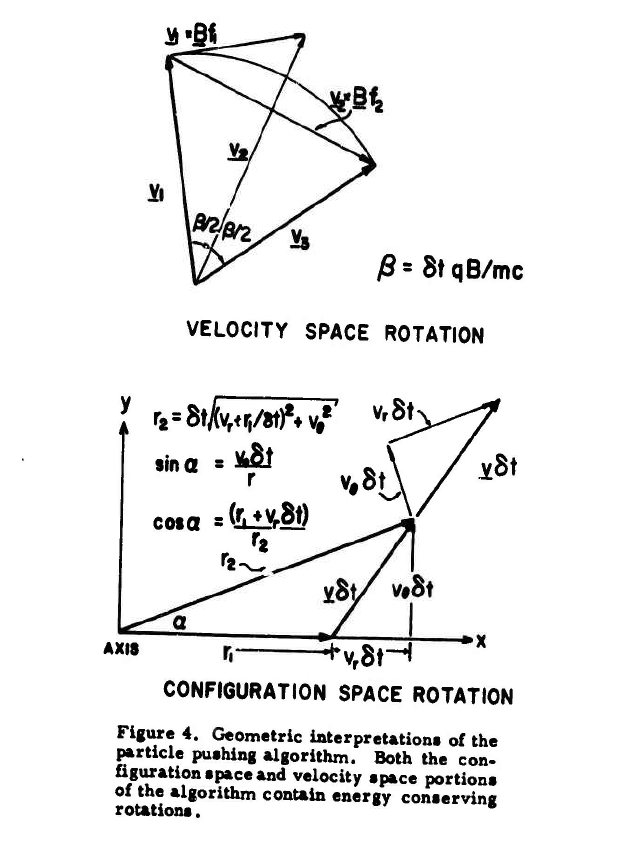
\includegraphics[width=0.6\textwidth]{pics/chap1/boris.png}
  \caption[Illustration of Boris velocity rotation]{Illustration of Boris
    velocity rotation, from \citep{boris_relativistic_1970}}
  \label{fig:boris-velocity-rotation}
\end{figure}


However one can see that an approximation was made in Boris pusher, namely the
average velocity vector between timesteps $i+1/2$ and $i-1/2$ is given by
equation \eqref{eq:boris-average-u}. However this is an approximation since
Boris pusher was derived with non-relativistic particle dynamics in mind.
\citet{vay_simulation_2008} pointed out that in the special case where
$\mathbf{E} + \mathbf{u}\times \mathbf{B}/c = 0$ the Boris pusher may introduce a
spurious force on the particles. A better average is simply given by
\begin{equation}
  \label{eq:vay-average-u}
  \bar{\mathbf{u}}^i = \frac{\mathbf{u}^{i-1/2} + \mathbf{u}^{i+1/2}}{2}
\end{equation}
However this means that the simple Boris scheme is no longer applicable. Vay
outlined a new scheme which is slightly more complicated but more accurate when
the Lorentz force of the particles is almost balanced by the electric force. The
procedure is as follows. One first define $\mathbf{p}'$ similar to that in Boris
pusher
\begin{equation}
  \label{eq:vay-p-prime}
  \mathbf{p}' = \mathbf{p}^{i-1/2} + q\Delta t\left( \mathbf{E}^i + \frac{\mathbf{u}^{i-1/2}}{2c}\times \mathbf{B}^i \right)
\end{equation}
then one can find $\mathbf{p}^{i+1/2}$ and $\gamma^{i+1/2}$ as follows:
\begin{align}
  \label{eq:vay-solution}
  \gamma^{i+1/2} &= \sqrt{\frac{\sigma + \sqrt{\sigma^2 + 4(\tau^2 + p_{*}^2)}}{2}} \\
  \mathbf{p}^{i+1/2} &= s \left[ \mathbf{p}' + (\mathbf{p}'\cdot \mathbf{t})\mathbf{t} + \mathbf{p}'\times \mathbf{t} \right]
\end{align}
where $\bm{\tau} = (q\Delta t/2c)\mathbf{B}^i$, $p_{*}=\mathbf{p}'\cdot\bm{\tau}/c$,
$\sigma = \gamma'^2-\tau^2$, $\gamma' = \sqrt{1 + p'^2/c^2}$, $\mathbf{t} =
\bm{\tau}/\gamma^{i+1/2}$, and $s = 1/(1 + t^2)$.

Since in the simulations of our interest, much of the plasma is both
relativistic and close to force-free, meaning that $\mathbf{E} +
\mathbf{u}\times \mathbf{B}/c$ is close to zero, it is important to use Vay
pusher to avoid spurious forces. Therefore in Aperture we use the Vay pusher
exclusively.

\subsection{Finite Difference Scheme for Maxwell Equations}
\label{sec:fd-maxwell}

In this section we outline how we use the fields $\mathbf{E}^{i}$ and
$\mathbf{B}^{i}$ to the compute their values at the next time step. The most
natural way is to use the traditional leapfrog method again
\begin{align}
  \label{eq:maxwell-leapfrog}
  \mathbf{E}^{i+1} &= \mathbf{E}^i + \Delta t (c\nabla\times \mathbf{B}^{i+1/2} - 4\pi \mathbf{j}^{i+1/2}) \\
  \mathbf{B}^{i+1/2} &= \mathbf{B}^{i-1/2} - \Delta t (c\nabla\times \mathbf{E}^i)
\end{align}
This scheme is stable as long as the time step $\Delta t$ satisfies the Courant
condition $\Delta t < \Delta x / c$ where $\Delta x$ is the smallest
grid spacing. However, one difficulty is that, in this scheme $\mathbf{E}$ and
$\mathbf{B}$ fields are not defined at the same time step, whereas in our
particle pusher \eqref{eq:leap-frog-particle} they are implicitly assumed to be
sampled at the same time step.

An improved method we employ is the semi-implicit field solver used by
\citep{haugboelle_photon-plasma:_2012}. We start from the following finite
difference equations:
\begin{align}
  \frac{\mathbf{E}^{i+1} -\mathbf{E}^{i}}{\Delta t} & = \nabla \times (
  \alpha \mathbf{B}^{i+1} + \beta \mathbf{B}^{i} ) -\mathbf{j}^{i+1/2}\\
  \frac{\mathbf{B}^{i+1} -\mathbf{B}^{i}}{\Delta t} & = - \nabla \times
  ( \alpha \mathbf{E}^{i+1} + \beta \mathbf{E}^{i} )
\end{align}
where $\alpha$ and $\beta$ are numerical parameters that determines
the ``implicitness'' of the scheme, with the constraint $\alpha +
\beta = 1$. If $\alpha \gtrsim 0.5$ then the scheme is unconditionally
stable. Bigger $\alpha$ leads to the damping of grid-scale waves,
which helps smoothing the solution.

To solve these equations, we can plug in the first equation into the second one
to eliminate $\mathbf{E}^{i+1}$, explicitly assuming $\nabla\cdot \mathbf{B} =
0$:
\begin{equation}
  \begin{split}
    (1 - \alpha^2\Delta t^2\nabla^2)\mathbf{B}^{i+1} &= \mathbf{B}^i + \alpha\beta \Delta t^2\nabla^2 \mathbf{B}^i \\
    &\phantom{=} -\Delta t\nabla\times \mathbf{E}^i + \alpha\Delta t^2\nabla\times \mathbf{j}^{i + 1/2}
  \end{split}
\end{equation}
Now this is an equation of $\mathbf{B}^{i+1}$ only. We can solve it by inverting
the operator $(1 - \alpha^2\Delta t\nabla^2)$ and apply it to the right hand side
\begin{equation}
  \label{eq:20}
  (1 - \alpha^2\Delta t^2\nabla^2)^{-1} = (1 + \alpha^2\Delta t^2\nabla^2 + (\alpha^2\Delta t^2\nabla^2)^2 + \dots)
\end{equation}
Provided $\Delta t$ is small enough, this series converges rapidly. Practically
we found that it is sufficient to terminate the series at around 4 terms, giving
a relative numerical error less than $10^{-8}$. Thus, although the Laplace
operator is a global operation and a global exchange of guard cell values is
required, the field solver is still significantly faster than the particle
pusher, rendering the overhead negligible.

One particular note is that if higher order numerical differential operators
were used in current deposition, then the same order of differential operators
should be used here in the field evolution, otherwise the exact charge
conservation will not be imposed. This is because we need the curl of
$\mathbf{B}$ to be divergence-free to numerical precision, which is only true
when the divergence and curl are evaluated to the same order of accuracy with
the same staggering structure (see section \ref{sec:discretization}).

\subsection{Coordinate Systems and Boundary Conditions}
\label{sec:coord-syst-sing}

Aperture supports the use of orthogonal curvilinear coordinate systems, which
basically means any parametrization of the Euclidean $\mathbb{R}^{3}$ that has a
diagonal metric. The coordinate system can be specified by three scale functions
$h_{i} = \sqrt{g_{ii}}$. Since the metric is diagonal, this contains all the
information of the metric.

The vector operations that we use in solving the Maxwell equations can be
written in terms of these scale functions:
\begin{align}
  \label{eq:vector-derivatives}
  \nabla f &= \frac{1}{h_{i}}\partial_{i}f \\
  \nabla \cdot \mathbf{V} &= \frac{1}{\prod_{k}h_{k}}\partial_i(V_i\prod_{j\neq i}h_{j}) \\
  \nabla \times \mathbf{V} &= \frac{1}{\prod_lh_l}\mathbf{e}_{i}\epsilon_{ijk}h_i\partial_j(h_kV_k)
\end{align}
where Einstein summation convention is assumed and repeated indices are summed
over (except in the product sign). Due to the general form of these equations,
it is straightforward to implement a general framework that works with vector
derivatives, that can take in any scale functions $h_{i}$.

Despite the designed flexibility, the main coordinate systems we support in the
actual code are Cartesian, cylindrical, spherical coordinates and some of their
variants. The scale functions of these coordinate systems are listed in table

\begin{table}[h]
  \centering
  \begin{tabular}{lccc}
    \hline
    Coordinate System & $h_1$ & $h_2$ & $h_3$ \\ \hline
    Cartesian ($x$, $y$, $z$) & 1 & 1 & 1 \\ \hline
    Cylindrical ($\rho$, $\theta$, $z$) & 1 & $\rho$ & 1 \\ \hline
    Spherical ($r$, $\theta$, $\phi$) & 1 & $r$ & $r\sin\theta$ \\ \hline
    Log spherical ($x$, $\theta$, $\phi$) & $e^x$ & $e^{x}$ & $e^x\sin\theta$ \\ \hline
  \end{tabular}
  \caption{Scale functions for coordinate systems implemented in Aperture}
  \label{tab:scale-functions}
\end{table}

An additional challenge in implementation of the coordinate systems
has to do with how boundary singularities are treated, which varies for
different coordinate systems. We will outline the treatment for the axis
boundary in the spherical coordinates here since it is the one implemented
first, and most relevant for the physics applications detailed in the later part
of the thesis.

For 2D spherical coordinates, axisymmetry means $\partial_{\phi} = 0$ in all
Maxwell equations. By symmetry, we automatically have on the axis
\begin{equation}
  E_{\theta} = E_{\phi} = B_{\theta} = B_{\phi} = 0
\end{equation}
simply because there is no preferred direction of these field components.
Furthermore, since we have $B_{\phi} = E_{\phi} = 0$ at the boundary for all
times, their time derivatives should vanish, which makes the following
conditions on the axis:
\begin{equation}
  \partial_r(rB_{\theta}) - \partial_{\theta}B_r = 0,\quad \partial_r(rE_{\theta}) - \partial_{\theta}E_{r} = 0
\end{equation}
Since $B_{\theta} = E_{\theta} = 0$ on the axis, so are their $r$
derivatives, therefore we have instead
\begin{equation}
  \partial_{\theta}B_r = \partial_{\theta}E_r = 0
\end{equation}
which is akin to a ``symmetric'' boundary condition for both $E_r$ and $B_r$.

The more important boundary condition is not on the fields, but on the
differential operators. Naively one might want to just apply the most
general differential operator on all points, and then correct for the
fields afterwards, but that approach is not ideal when higher order
differential operators are involved, nor is it appropriate when one
wants to chain several differential operators together to evaluate,
say, $\nabla\times(\nabla\times \mathbf{B})$.

Therefore let us reformulate the problem into finding the appropriate
boundary condition for $\nabla\times \mathbf{E}$ and $\nabla\times
\mathbf{B}$ at the axis $\theta = 0$, $\pi$. The differential operator
looks like the following:
\begin{equation}
  \begin{split}
    \nabla\times \mathbf{E} &= \hat{\mathbf{r}}\frac{1}{r\sin\theta}\partial_{\theta}^-\sin\theta E_{\phi} \\
    &- \hat{\bm{\theta}}\frac{1}{r}\partial_r^-rE_{\phi} \\
    &+ \hat{\bm{\phi}}\left( \frac{1}{r}\partial_r^-rE_\theta - \frac{1}{r}\partial_{\theta}^-E_r \right)
  \end{split}
\end{equation}
And similar for $\mathbf{B}$. Note that all differential operators are
$\partial^-$ in the case of $\nabla\times \mathbf{E}$, and
$\partial^+$ in the case of $\nabla\times \mathbf{B}$. Near the axis,
the problematic terms are the $\partial_{\theta}$ derivatives. That
means the $\partial_{\theta}\sin\theta E_{\phi}$ term and the
$\partial_{\theta}E_r$ term.

For the later, we have the powerful condition that right on the axis
$\partial_{\theta}E_r = 0$. In fact, we have $(\nabla\times
\mathbf{E})_{\phi} = 0$ at the axis boundary. For $\nabla\times
\mathbf{E}$, it is directly evaluated on the boundary, therefore we
impose the above condition directly on the boundary cell. For the cell
in the box directly next to the boundary, we use the modified
one-sided 4th order scheme:
\begin{equation}
  \label{eq:1-sided-4th-order}
  \partial_{\theta}^-E_{i,j}^r = \frac{1}{\Delta r}\left[-\frac{11}{24} E_{i,j}^{r} + \frac{17}{24}E_{i+1,j}^{r} + \frac{3}{8}E^{r}_{i+2,j} - \frac{5}{24}E^{r}_{i+3,j} + \frac{1}{24}E^r_{i+4,j} )\right]
\end{equation}
Since $E_{\phi}$ and $E_r$ are similarly staggered in the $\theta$
direction, same formula applies. Points further into the box do not
feel the presence of the boundary.

For the former term it is a bit tricky, since the coefficient
$1/r\sin\theta$ vanishes at the axis. A limit analysis reveals that
\begin{equation}
  \lim_{\theta\to 0}\frac{1}{r\sin\theta}\partial_{\theta}\sin\theta E_{\phi} = \frac{2\partial_{\theta}E_{\phi}}{r}
\end{equation}
And since $(\nabla\times \mathbf{E})_r$ is directly evaluated on the
axis boundary, we need to use the above formula to compute its
value. When computing the derivative $\partial_{\theta}E_r$, we can
use an even more extreme version of the 4th-order one-sided
derivative:
    % return (-f1 * 31.0 / 8.0 + f2 * 229.0 / 24.0 - f3 * 75.0 / 8.0 + f4 * 37.0 / 8.0 - f5 * 11.0 / 12.0) / delta;
\begin{equation}
  \partial_{\theta}^-E_{i,j}^\phi = \frac{1}{\Delta r}\left[-\frac{31}{8} E_{i+1,j}^{\phi} + \frac{229}{24}E_{i+2,j}^{\phi} - \frac{75}{8}E^{\phi}_{i+3,j} + \frac{37}{8}E^{\phi}_{i+4,j} - \frac{11}{12}E^\phi_{i+5,j} )\right]
\end{equation}
However, there is one piece of information we can use, which is the
fact that $E_{\phi} = 0$ on the boundary. If taken this condition into
account, then we can reduce the above equation into the modified
one-sided derivative:
\begin{equation}
  \partial_{\theta}^-E_{i,j}^\phi = \frac{1}{\Delta r}\left[\frac{35}{8} E_{i+1,j}^{\phi} - \frac{35}{24}E_{i+2,j}^{\phi} + \frac{21}{40}E^{\phi}_{i+3,j} - \frac{5}{56}E^{\phi}_{i+4,j} )\right]
\end{equation}

For $\nabla\times \mathbf{B}$ the analysis is similar. However, due to
the difference in staggering scheme, different components are
evaluated at the boundary. Therefore different boundary considerations
apply. For the $\partial_{\theta}B_r$ term, since it is not evaluated
directly on the boundary, we need only use the one-sided derivative
\eqref{eq:1-sided-4th-order} for the point closest to the boundary.

For the $\partial_r(\sin\theta B_{\phi})/r\sin\theta$ term, again it
is not evaluated directly on the boundary, therefore we only need to
use \eqref{eq:1-sided-4th-order} on the point closest to the boundary,
similar to the above term.

The analysis up to this point completely fixes $\nabla\times
\mathbf{E}$ and $\nabla\times \mathbf{B}$ at the axis boundary. Even
if our $\theta$ boundary is not taken to be exactly at $\theta = 0$,
$\pi$, the above conditions should still approximately hold. Plus,
since the evaluation of the curl does not need anything from the ghost
cells, we can evaluate $\nabla\times(\nabla\times \mathbf{B})$ with no
problem.

If we want to implement the semi-implicit scheme, then we need to fix
the boundary condition for the differential operator $\nabla\cdot
\mathbf{B}$ at the axis as well. We have
\begin{equation}
  \begin{split}
        \nabla\cdot \mathbf{B} &= \frac{1}{r^2}\partial_r^-(r^2B_r) + \frac{1}{r\sin\theta}\partial_{\theta}^-(\sin\theta B_{\theta}) \\
        &= \frac{1}{r^3\sin\theta}\left[ \partial_x^-(r^2\sin\theta B_r) + \partial_{\theta}^-(r^2\sin\theta B_{\theta}) \right]
    \end{split}
\end{equation}
The second line is written out explicitly in log-spherical
coordinates. Both terms present a challenge since $\sin\theta$ is zero
on the axis. The second term reduces to
$2\partial_{\theta}B_{\theta}/r$ similar to what happens before, and
can be dealt with using the modified one-sided derivative
\eqref{eq:14}. This is actually the property of the
$\partial_{\theta}^-$ operator. The first term need to be evaluated
with $\sin\theta$ moved out from the derivative, and this needs to be
done in the code by hand as a special case.

Lastly we have the gradient operator. We actually have two different
versions depending on whether $f$ is evaluated at the center of the
cell or at the corner of the cell. If we call the former $f^-$ and the
latter $f^+$, then
\begin{equation}
  \nabla f^- = \hat{\mathbf{r}}\partial_r^-f + \hat{\bm{\theta}}\frac{1}{r}\partial_{\theta}^-f
\end{equation}
and similar for $f^+$. Obviously $\nabla\cdot \mathbf{B}$ belongs to $f^+$.
% and the two components have the same stagger structure as $\mathbf{B}$
% if $f = \nabla\cdot \mathbf{B}$.
% The problem near the axis arises in the second term in the $\theta$
% derivative.
Since the derivative involved is $\partial^+$ and therefore not
evaluated on the axis, simply using \eqref{eq:1-sided-4th-order} near
the axis will fix the problem.


\subsection{Radiative Transfer}
\label{sec:radiative-transfer}

A significant feature of Aperture compared to traditional PIC codes is the
inclusion of various radiative transfer mechanisms that are important in
high-energy astrophysics. In this section we list the supported physical
processes and outline how we model them in the code.

\subsubsection{Channels for pair creation}
\label{sec:instant-pair}

In the magnetosphere of neutron stars, energetic electrons or positrons can
induce vacuum breakdown and create $e^{\pm}$ pairs. This is usually a 2-step
process. First, a high energy photon ($E_\mathrm{ph} > 2m_{e}c^2$) is emitted
from the energetic particle, and the photon will then convert into a pair of
$e^{\pm}$. In rotation powered pulsars, the first process is believed to be
mainly from curvature radiation from electrons accelerated to Lorentz factors
$\gamma \gtrsim 10^{8}$. % TODO: refer to the intro section
However in magnetars where the magnetic field is strong, the energetic photons
mainly come from resonantly up scattered X-ray photons from either the thermal
emission from the surface of the star, or from synchrotron emission of the
plasma in the magnetic field.

Aperture models both kinds of high-energy photon emission with a threshold
condition and an emission rate.


\subsubsection{Synchrotron and general radiative loss}
\label{sec:synchrotron-loss}

\subsubsection{Radiative drag due to resonant scattering}
\label{sec:resonant-scattering}


% \subsection{Organization of the Code}
% \label{sec:code-organization}

\subsection{Units}
\label{sec:pic-units}

A computer simulation is ignorant of the physical units of the dynamic
variables, therefore one should choose a unit for all physical quantities, such
that in the code all quantities are pure numbers. It is to our benefit to choose
a unit system that is most natural to the problem and in which the dynamic
equations take the simplest dimensionless form. We try to establish that in this
section.

The primary goal of the code is to simulate an isolated neutron star, therefore
the natural length scale is the stellar radius, and there is no other length
scale {\it a priori}. Naturally, the time scale of the problem would be the
light-crossing time of the star. Therefore we define the dimensionless length
and time using the following equations (in all the following equations, a tilde
on the symbol means the dimensionless version):
\begin{equation}
  r = \tilde{r}R_{*},\quad t = \tilde{t}\frac{R_{*}}{c},\quad \omega = \tilde{\omega}\frac{c}{R_{*}}
\end{equation}
The radius $r = 1$ shows up mainly as the lower boundary of most of our
simulations.

Once we add rotation of the star and magnetic field, two important frequencies
show up in this problem that can then be written in dimensionless units:
\begin{equation}
  \tilde{\Omega} = \frac{\Omega R_{*}}{c},\qquad \tilde{\omega}_B = \frac{\omega_BR_{*}}{c} = \frac{e B_0R_{*}}{mc^2}
\end{equation}
where $\Omega$ is the rotation angular frequency, equal to $2\pi / P$ where $P$ is the period of rotation, and $B_0$ is the surface magnetic field at the pole. Given a pulsar with certain radius, these two are the dimensionless parameters that will govern the simulation, and hence the physical behavior of the system.

We want to define a unit for charge density. This can be done by relating the
plasma frequency, a third frequency in the problem, with the local corotation
charge density $\rho_\mathrm{GJ}$. We define the reference plasma frequency at every
point as
\begin{equation}
  \omega_p^2 = \frac{4\pi \rho_\mathrm{GJ}e}{m}
\end{equation}
then we can define a version of dimensionless Goldreich-Julian density, or any charge density
\begin{equation}
  \rho_\mathrm{GJ} = \frac{m \tilde{\omega}_p^2 c^2}{4\pi e R_{*}^2} = \tilde{\rho}_\mathrm{GJ} \frac{mc^2}{4\pi eR_{*}^2}
\end{equation}
Note the real plasma frequency will depend on the actual plasma number density
at the point of interest and will in general be different from what we call
$\omega_p$ above. However, it is still useful to determine such a characteristic
plasma frequency for reference. What the above equation says is that, by
choosing these units we make $\tilde{\rho} = \tilde{\omega}_p^2$. Especially,
there is a simple relationship between the three characteristic frequencies in
the problem, if we define $\rho_{GJ} = \Omega B_0 / 2\pi c$:
\begin{equation}
  \frac{m \omega_p^2}{4\pi e} = \frac{\Omega B_0}{2\pi c} \quad \Longrightarrow \quad \tilde{\omega}_p^2 = 2\tilde{\Omega} \tilde{\omega}_B
\end{equation}
Therefore, specifying the numerical values of $\tilde{\Omega}$ and
$\tilde{\omega}_B$ automatically determines the characteristic plasma frequency
in the problem.

With the above choices, we can work out the dimensionless electric and magnetic
fields. Gauss's law gives
\begin{equation}
  \nabla\cdot \mathbf{E} = 4\pi \rho \quad \Longrightarrow \quad \frac{\Delta E}{\Delta \tilde{r} R_{*}} = \tilde{\rho} \frac{m c^2}{e R_{*}^2} \quad \Longrightarrow \quad E = \tilde{E}\frac{m c^2}{e R_{*}}
\end{equation}
and similarly
\begin{equation}
    B = \tilde{B}\frac{m c^2}{e R_{*}}
\end{equation}
Note that this means $B$ and $\omega_B$ has the same dimensionless form,
therefore $\tilde{B}_0 = \tilde{\omega}_B$.

Under these units, Maxwell equations look like
\begin{equation}
  \partial_t \tilde{\mathbf{E}} = \tilde{\nabla}\times \tilde{\mathbf{B}} - \tilde{\mathbf{j}},\quad \partial_t \tilde{\mathbf{B}} = - \tilde{\nabla}\times \tilde{\mathbf{E}}
\end{equation}
and the particle equations of motion look like
\begin{equation}
  \frac{d \tilde{\mathbf{p}}}{d \tilde{t}} = \tilde{\mathbf{E}},\quad \frac{d \tilde{\mathbf{r}}}{d \tilde{t}} = \tilde{\mathbf{u}} = \frac{\tilde{p}}{\sqrt{1 + \tilde{p}^2}} \tilde{\mathbf{p}}
\end{equation}

Up to now, all the numerical parameters we have introduced are $\tilde{\Omega}$
and $\tilde{\omega}_B$, and they specify all the physics of the system. For
simulation purposes, one needs to rescale both of these parameters to bring the
size of the system into computable regime. However, one more numerical parameter
is required for interpolating between the particle charge and the charge density
on the grid, namely the charge of an individual macro particle. Since in PIC
there is no way to simulate realistic plasma of order $10^{20+}$ particles, one
needs to use one single macro particle to represent a collection of physical
particles. A macro particle has the same charge-to-mass ratio as a physical
particle, but has more charge (therefore mass). The way we choose the charge per
particle is to normalized it such that our characteristic charge density
$\rho_\mathrm{GJ}$ would correspond to a certain manageable number of particles $N_p$
per cell.

The way we compute charge density is to iterate over all particles and deposit
onto a single cell:
\begin{equation}
    \rho_c = \frac{\sum e_p W(\mathbf{r}_p, \mathbf{r}_c)}{\Delta V}
\end{equation}
where $e_p$ is the charge per macro particle, $S$ is a shape factor depending on
particle position $\mathbf{r}_p$ and grid point position $\mathbf{r}_c$, and
$\Delta V$ is the size of the cell. Assuming every particle has the same charge
$e$, and there are $N_p$ particles in the cell, up to a form factor, we have
\begin{equation}
    \rho = \frac{e N_p}{\Delta V} = \frac{e N_p}{\Delta \tilde{V} R_{*}^{3}} = \tilde{\rho}\frac{mc^2}{4\pi eR_{*}^2}, \quad \tilde{\rho} = \frac{\tilde{e}N_p}{\Delta \tilde{V}}
\end{equation}
so we can identify the dimensionless charge per particle
\begin{equation}
    \tilde{e} = e \frac{4\pi e}{mc^2R_{*}}
\end{equation}
Note that $e$ appears twice on the right hand side. This is because we treat
$e/m$ as a physical constant, therefore $4\pi e / mc^2R_{*}$ is a physical
constant which is fixed as soon as we choose the physical size of the star. We'd
like to choose $\tilde{e}$ such that $N_p$ particles per cell corresponds to the
characteristic charge density $\rho_\mathrm{GJ}$:
\begin{equation}
    \tilde{\rho} \sim \frac{\tilde{e} N_p}{\Delta \tilde{V}} \sim \tilde{\rho}_\mathrm{GJ} \quad \Longrightarrow \quad \tilde{e} = \frac{2\tilde{\Omega} \tilde{B}\Delta \tilde{V}}{N_p}
\end{equation}

One technical aspect about the numerical value $\tilde{e}$ in the code is that,
every time we use $\tilde{e}$, we actually use the combination $\tilde{e}/\Delta
\tilde{V}$, which shows up in charge/current deposition. Therefore it is not
necessary to carry $\Delta \tilde{V}$ around. We simply remove it from the
definition of $\tilde{e}$, and don't divide by $\Delta \tilde{V}$. Also a factor
of 2 is not that important, so in the code the actual value of $\tilde{e}$ is
taken to be
\begin{equation}
    \tilde{e} = \frac{\tilde{\Omega} \tilde{B}_0}{N_{p}}
\end{equation}

To summarize, the numerical parameters in our simulation are $\tilde{\Omega}$,
$\tilde{\omega}_B$ (or equivalently $\tilde{B}_{0}$), and $\tilde{e}$ (or
equivalently $N_p$ after specifying cell size). This completely specifies the
computational problem. In order to translate this numerical simulation to
reality, we need to specify $R_{*}$ in physical units (e.g.\ $10^6\,
\mathrm{cm}$), and multiply the dimensionless units by their physical units to
get the realistic values. The dimensionful units are summarized below (subscript
$*$ means that these are the dimensionful units for the physical quantity in
question, e.g.\ $E = \tilde{E} E_*$)
\begin{align}
  r_{*} &= R_{*} = R_6\, 10^6\, \mathrm{cm} \\
  t_{*} &= R_{*} / c = R_6\,3.33\times 10^{-5}\, \mathrm{s} \\
  E_{*} &= B_{*} = \frac{mc^2}{eR_{*}} = R_6^{-1}\, 2.08\times 10^{-5}\, \mathrm{statV/cm(G)} \\
  \rho_{*} &= \frac{mc^2}{4\pi eR_{*}^2} = R_{6}^{-2}\, 1.66\times 10^{-12}\, \mathrm{statC/cm^3} \\
  j_{*} &= \frac{mc^3}{4\pi eR_{*}^2} = R_{6}^{-2}\, 4.96\times 10^{-2}\, \mathrm{statC/cm^2\cdot s}  \\
  e_{*} &= \frac{mc^2R_{*}}{4\pi e} = R_6\, 1.66\times 10^6\, \mathrm{statC} \\
  g_{*} &= R_{*}c^2 = R_6\, 9.0\times 10^{26}\, \mathrm{m^3s^{-2}} \\
  p_{*} &= mc
\end{align}

\section{Aperture}

\section{Test Problems}
\label{sec:test-problems}
% This section we present some tests that show the validity of the
% code, in several coordinate systems, and in several physical scenarios

\section{Example Applications}
\label{sec:example-applications}
% This section we present some of toy physical models that we can
% simulate using this code, including axisymmetric pulsar (briefly),
% magnetar, twisted cylinder, Gruzinov problem, etc.

\section{Discussions and Remarks}
\label{sec:discussions}

% Local Variables:
% TeX-master: "../thesis"
% zotero-collection: #("16" 0 2 (name "Thesis"))
% End:
